\documentclass[runningheads]{llncs}

% ── Packages ───────────────────────────────────────────────────────────────────
\usepackage[T1]{fontenc}
\usepackage{graphicx}
\usepackage{amsmath,amssymb}
\usepackage{booktabs}
\usepackage{multirow}
\usepackage{array}
\usepackage{url}
\usepackage{hyperref}
\usepackage{xcolor}
\usepackage[capitalise]{cleveref}

% Convenience macro for TODO notes during drafting
\newcommand{\todo}[1]{\textcolor{red}{[TODO: #1]}}

\begin{document}

% ── Title ──────────────────────────────────────────────────────────────────────
\title{Beyond Gradient-Based Attacks: Adversarial Robustness and Explainability
Stability in Cybersecurity Classifiers}

\titlerunning{Adversarial Robustness and Explainability Stability}

\author{Mona Rajhans\inst{1} \and
        Vishal Khawarey\inst{2}}

\authorrunning{M. Rajhans and V. Khawarey}

\institute{Palo Alto Networks, Santa Clara, CA, USA\\
           \email{mrajhans@paloaltonetworks.com}
           \and
           Quicken Inc., Menlo Park, CA, USA\\
           \email{vishalkk@gmail.com}}

\maketitle

% ── Abstract ──────────────────────────────────────────────────────────────────
\begin{abstract}
Adversarial attacks on machine learning classifiers used in cybersecurity
represent a growing practical threat, yet most empirical studies focus on
gradient-based attacks against neural networks evaluated on image benchmarks.
In this work we extend our prior study~\cite{khawarey2026empirical} to provide
a comprehensive empirical analysis of adversarial robustness and explainability
stability for three classifier families---Multi-Layer Perceptron~(MLP), Random
Forest~(RF), and XGBoost---across three tabular cybersecurity datasets: phishing
URL detection, UNSW-NB15 network intrusion, and NF-ToN-IoT IoT traffic.
Beyond gradient-based attacks~(FGSM, PGD), we evaluate three black-box attack
methods~(ZOO, Square Attack, HopSkipJump) applicable to non-differentiable tree
models.  We introduce the \emph{Explainability Stability Index}~(ESI), a scalar
metric computed from TreeSHAP attribution drift that measures how stable a
model's explanations remain under adversarial perturbation.  Our key finding is
that prediction robustness and explanation stability are \emph{decoupled}:
XGBoost achieves near-perfect robustness under ZOO~(RI\,$\approx$\,0.98) yet
exhibits very low explanation stability~(ESI\,$\approx$\,0.06--0.11).
We further show that ZOO produces degenerate gradient estimates against XGBoost,
and that attack-method selection is not model-agnostic---Square Attack reveals
vulnerability hidden by ZOO.  A step-size ablation for PGD explains a previously
unreported anomaly on normalised tabular data.  Experiment code and result tables
are publicly available~\cite{khawarey2026code}.

\keywords{Adversarial robustness \and Explainability drift \and SHAP \and
TreeSHAP \and Cybersecurity \and Intrusion detection \and XGBoost \and
Random Forest \and Black-box attacks \and Explainability Stability Index}
\end{abstract}

% ══════════════════════════════════════════════════════════════════════════════
\section{Introduction}
\label{sec:intro}
% ══════════════════════════════════════════════════════════════════════════════

Machine learning classifiers are widely deployed in cybersecurity pipelines---for
phishing URL detection, network intrusion detection, and IoT anomaly
detection---where both accurate predictions and trustworthy explanations are
required for operational use.  Adversarial attacks, which apply small deliberate
perturbations to inputs to cause misclassification, pose a dual threat: they
degrade prediction accuracy and, as we demonstrate here, simultaneously destabilise
the SHAP-based explanations that security analysts rely on to understand model
decisions.

Prior work on adversarial robustness has focused almost exclusively on image
classifiers and gradient-based attacks~\cite{goodfellow2015explaining,madry2018towards},
with limited attention to the structured tabular data characteristic of network
security~\cite{grosse2017adversarial,yang2020defending}.  A further gap is that
most studies evaluate a single model family---typically deep neural networks---and
a single attack class, providing an incomplete picture of cross-model robustness.
Our conference paper~\cite{khawarey2026empirical} addressed the tabular-data gap
for MLP classifiers, introducing the Robustness Index~(RI) and characterising
SHAP attribution drift under FGSM and PGD.  Reviewer feedback on that work called
for tree-based classifiers, additional attack methods, and a rigorous explanation
of the PGD\,$<$\,FGSM anomaly observed in the results.

This extended study addresses all three requests and adds further contributions.
Specifically, we make the following new contributions beyond~\cite{khawarey2026empirical}:

\begin{itemize}
  \item \textbf{Tree ensemble evaluation.}  RF and XGBoost are evaluated alongside
    the MLP, representing the model family most commonly deployed in production
    cybersecurity systems.
  \item \textbf{Black-box attack framework.}  Three black-box attacks---ZOO,
    Square Attack, and HopSkipJump---are implemented and evaluated, enabling
    attack of non-differentiable tree models.
  \item \textbf{Explainability Stability Index (ESI).}  A new scalar metric
    computed from TreeSHAP drift, directly comparable to RI on the same scale.
  \item \textbf{Third dataset.}  NF-ToN-IoT is added as an IoT intrusion
    detection domain, providing cross-domain validation.
  \item \textbf{ZOO degeneracy finding.}  We show empirically that ZOO produces
    near-degenerate results on XGBoost (RI\,=\,0.97) due to its piecewise-constant
    prediction surface, while Square Attack reveals genuine vulnerability
    (RI\,=\,0.36), exposing a methodological risk in attack-method selection.
  \item \textbf{PGD step-size ablation.}  A controlled ablation confirms the
    PGD\,$<$\,FGSM anomaly is a hyperparameter sensitivity artifact on
    z-score normalised tabular data.
\end{itemize}

The remainder of this paper is structured as follows.
\Cref{sec:related} reviews related work.
\Cref{sec:formulation} defines the threat model and metrics~(RI, ESI).
\Cref{sec:attacks} describes the five attack methods.
\Cref{sec:setup} details the experimental setup.
\Cref{sec:base} summarises the base MLP study from~\cite{khawarey2026empirical}.
\Cref{sec:trees} presents the tree model extension.
\Cref{sec:toniot} covers the NF-ToN-IoT dataset.
\Cref{sec:pgd} presents the PGD ablation.
\Cref{sec:discussion} discusses attack realism and ESI implications.
\Cref{sec:conclusion} concludes.

% ══════════════════════════════════════════════════════════════════════════════
\section{Related Work}
\label{sec:related}
% ══════════════════════════════════════════════════════════════════════════════

\paragraph{Adversarial robustness.}
Biggio et al.~\cite{biggio2013evasion} established the foundational evasion-attack
framework for machine learning.  Goodfellow et al.~\cite{goodfellow2015explaining}
introduced FGSM, and Madry et al.~\cite{madry2018towards} extended it to iterative
PGD, now a standard robustness benchmark.  Carlini and
Wagner~\cite{carlini2017towards} proposed optimisation-based attacks demonstrating
limits of adversarial training.  Cohen et al.~\cite{cohen2019certified} introduced
randomised smoothing for certified robustness.  Fawzi et
al.~\cite{fawzi2018analysis} analysed theoretical robustness bounds.

\paragraph{Black-box attacks.}
Chen et al.~\cite{chen2017zoo} introduced ZOO, which approximates gradients via
finite differences without access to model internals.  Andriushchenko et
al.~\cite{andriushchenko2020square} proposed Square Attack, a score-based method
relying only on loss values.  Chen et al.~\cite{chen2020hopskipjump} proposed
HopSkipJump, a decision-based attack requiring only predicted labels.

\paragraph{Adversarial attacks in cybersecurity.}
Papernot et al.~\cite{papernot2016limitations} demonstrated adversarial
vulnerability of deep networks in security settings.  Grosse et
al.~\cite{grosse2017adversarial} applied adversarial perturbations to malware
classifiers.  Yang et al.~\cite{yang2020defending} studied defence strategies
for cybersecurity DNNs.  These works focus primarily on neural networks; tree
ensemble robustness under black-box attacks remains less studied.

\paragraph{Explainability and its stability.}
Lundberg and Lee~\cite{lundberg2017unified} introduced SHAP as a unified
attribution framework.  Lundberg et al.~\cite{lundberg2020treeshap} extended
SHAP to tree models via TreeSHAP, enabling exact attributions.  Slack et
al.~\cite{slack2020fooling} showed LIME and SHAP explanations can be manipulated
by adversarial inputs, motivating quantitative stability measurement.
Agarwal et al.~\cite{agarwal2022openxai} introduced OpenXAI with metrics
including RIS and ROS for explanation faithfulness; our ESI is orthogonal,
measuring explanation stability under adversarial drift rather than faithfulness
to model internals.

% ══════════════════════════════════════════════════════════════════════════════
\section{Problem Formulation and Metrics}
\label{sec:formulation}
% ══════════════════════════════════════════════════════════════════════════════

\subsection{Threat Model}

We consider an attacker with access to a trained classifier $f: \mathcal{X}
\rightarrow \mathcal{Y}$ who seeks to cause misclassification by adding a
perturbation $\delta$ bounded in the $L_\infty$ norm: $\|\delta\|_\infty \leq
\varepsilon$.  For white-box attacks (FGSM, PGD), the attacker has access to
model gradients.  For black-box attacks (ZOO, Square Attack, HopSkipJump), the
attacker has access only to model predictions or prediction probabilities.
We focus on evasion attacks at inference time; poisoning and model-extraction
attacks are out of scope.

\subsection{Robustness Index (RI)}

The Robustness Index, introduced in~\cite{khawarey2026empirical}, summarises
accuracy degradation over the perturbation budget $\varepsilon$ as a single scalar:

\begin{equation}
  \mathrm{RI} = \frac{1}{\varepsilon_{\max}}
  \int_0^{\varepsilon_{\max}} \mathrm{Acc}(\varepsilon)\, d\varepsilon
  \label{eq:ri}
\end{equation}

where $\mathrm{Acc}(\varepsilon)$ is the classifier accuracy under attack at
perturbation budget $\varepsilon$.  RI lies in $[0, 1]$; higher values indicate
greater robustness.  In practice the integral is approximated via the trapezoidal
rule over a grid of $\varepsilon$ values.

\subsection{Explainability Stability Index (ESI)}

We introduce ESI as the explanation-domain analogue of RI.  Let
$\phi_i(\mathbf{x})$ denote the SHAP attribution of feature $i$ for input
$\mathbf{x}$.  The per-feature attribution drift at perturbation budget
$\varepsilon$ is:

\begin{equation}
  \Delta\Phi_i(\varepsilon) =
  \mathbb{E}\!\left[\,\left|\phi_i(\mathbf{x}_{\mathrm{adv}})
  - \phi_i(\mathbf{x})\right|\,\right]
  \label{eq:drift}
\end{equation}

where the expectation is over the test set and $\mathbf{x}_{\mathrm{adv}}$ is
the adversarial example at budget $\varepsilon$.  The mean drift across all
features is $\bar{D}(\varepsilon) = \frac{1}{d}\sum_i \Delta\Phi_i(\varepsilon)$.
ESI is then:

\begin{equation}
  \mathrm{ESI} = 1 - \frac{1}{\varepsilon_{\max}}
  \int_0^{\varepsilon_{\max}}
  \frac{\bar{D}(\varepsilon)}{\bar{D}(\varepsilon_{\max})}\, d\varepsilon
  \label{eq:esi}
\end{equation}

Normalising by $\bar{D}(\varepsilon_{\max})$ places ESI on the same $[0,1]$
scale as RI.  Higher ESI indicates that explanations remain stable under attack.
For tree models, SHAP values are computed exactly via TreeSHAP~\cite{lundberg2020treeshap};
for the MLP, a kernel approximation is used.

% ══════════════════════════════════════════════════════════════════════════════
\section{Attack Methods}
\label{sec:attacks}
% ══════════════════════════════════════════════════════════════════════════════

\paragraph{FGSM.}  The Fast Gradient Sign Method~\cite{goodfellow2015explaining}
computes a single-step perturbation in the direction of the loss gradient:
$\mathbf{x}_{\mathrm{adv}} = \mathbf{x} + \varepsilon\,\mathrm{sign}
(\nabla_\mathbf{x}\mathcal{L}(f(\mathbf{x}), y))$.

\paragraph{PGD.}  Projected Gradient Descent~\cite{madry2018towards} iterates
FGSM with step size $\alpha$ and projects back to the $L_\infty$ ball after each
step.  We use 10 steps with $\alpha=0.01$ (default) and vary $\alpha$ in the
ablation of \cref{sec:pgd}.

\paragraph{ZOO.}  ZOO~\cite{chen2017zoo} approximates the gradient via
symmetric finite differences:
$\hat{g}_j = (\mathcal{L}(\mathbf{x} + \delta_j \mathbf{e}_j, y)
- \mathcal{L}(\mathbf{x}, y)) / \delta_j$,
then applies the FGSM sign update.  It requires only black-box loss access.

\paragraph{Square Attack.}  Square Attack~\cite{andriushchenko2020square} is a
score-based method that applies random square-shaped perturbations, accepting
updates that increase the adversarial loss.  We use 150 queries with initial
perturbation probability $p_{\mathrm{init}} = 0.5$.

\paragraph{HopSkipJump.}  HopSkipJump~\cite{chen2020hopskipjump} is a
decision-based attack requiring only predicted class labels.  It alternates
between a binary search to find the decision boundary and a gradient estimation
step via Monte Carlo sampling.  We use 8 iterations with 20 gradient samples.

% ══════════════════════════════════════════════════════════════════════════════
\section{Experimental Setup}
\label{sec:setup}
% ══════════════════════════════════════════════════════════════════════════════

\paragraph{Datasets.}
Three tabular cybersecurity datasets are used.
\textit{Phishing URL}~\cite{phishing_kaggle}: 10{,}000 samples, 48 binary/ternary
URL-structure features, balanced classes.
\textit{UNSW-NB15}~\cite{moustafa2015unsw}: 175{,}341 network flow records, 40
features (categorical encoded), binary normal/attack label.
\textit{NF-ToN-IoT}~\cite{sarhan2021nftoniot}: 1{,}157{,}994 NetFlow~v2 records,
10 features; we sample 20{,}000 benign and 20{,}000 attack flows using stratified
batch streaming to avoid loading the full file into memory.
All features are z-score normalised using training-set statistics.

\paragraph{Models.}
We evaluate three classifiers: an MLP with two hidden layers (64, 32 units, ReLU,
Adam, 20 epochs), a Random Forest (100 trees, max depth 8), and XGBoost
(100 trees, max depth 5, learning rate 0.05).  All models use fixed random seeds
for reproducibility.

\paragraph{Attack evaluation protocol.}
Perturbation budgets $\varepsilon \in \{0, 0.033, 0.067, \ldots, 0.30\}$ (10
values).  FGSM and PGD are applied to the MLP on the full test set.  Black-box
attacks (ZOO, Square Attack, HopSkipJump) are applied to RF and XGBoost on a
stratified subsample of 300 test examples (120 for HopSkipJump, which is
query-intensive).  ESI is computed on a 256-sample stratified subset.

% ══════════════════════════════════════════════════════════════════════════════
\section{Base Study: MLP under White-Box Attacks}
\label{sec:base}
% ══════════════════════════════════════════════════════════════════════════════

This section summarises results from our conference
paper~\cite{khawarey2026empirical}, reproduced here for reference.  All figures
and tables in this section are adapted from~\cite{khawarey2026empirical}.

The MLP achieves clean accuracy of 0.857 on Phishing and 0.774 on UNSW-NB15.
Under FGSM, accuracy degrades monotonically with $\varepsilon$; RI values are
0.610 (Phishing) and 0.692 (UNSW-NB15).  Under PGD~($\alpha=0.01$, 10 steps),
accuracy degrades less steeply, yielding higher RI values of 0.725 (Phishing)
and 0.733 (UNSW-NB15).  This counterintuitive PGD\,$<$\,FGSM result is explained
in \cref{sec:pgd}.  Adversarial training with FGSM perturbations at
$\varepsilon=0.05$ improves RI by approximately 0.08--0.12 on both datasets at
the cost of a 2--4\% drop in clean accuracy.

SHAP attribution drift increases monotonically with $\varepsilon$ across all
features.  URL-structure features (e.g.\ \texttt{PctExtNullSelfRedirectHyperlinks},
\texttt{UrlLengthRT}) show the highest drift on Phishing;
\texttt{dttl} and \texttt{ct\_dst\_sport\_ltm} are the most drift-prone on UNSW-NB15.

% ══════════════════════════════════════════════════════════════════════════════
\section{Tree Ensemble Extension: Black-Box Attacks and ESI}
\label{sec:trees}
% ══════════════════════════════════════════════════════════════════════════════

\subsection{Results: Phishing and UNSW-NB15}

Table~\ref{tab:master} presents RI and ESI for all models, datasets, and attack
methods.  Key observations are discussed below.

\begin{table}[t]
\caption{Robustness Index (RI) and Explainability Stability Index (ESI) across
all models, datasets, and attack methods. Higher is better for all metrics.
``---'' indicates the attack is inapplicable to that model family.
$^\dagger$FGSM/PGD for MLP; ZOO for tree models.}
\label{tab:master}
\centering
\small
\begin{tabular}{llccccccc}
\toprule
\multirow{2}{*}{Dataset} & \multirow{2}{*}{Model} &
  \multirow{2}{*}{Clean} &
  \multicolumn{4}{c}{Robustness Index (RI)} &
  \multirow{2}{*}{ESI} \\
\cmidrule(lr){4-7}
& & Acc & FGSM/ZOO$^\dagger$ & PGD & Square & HSJ & \\
\midrule
\multirow{3}{*}{Phishing}
  & MLP  & 0.857 & 0.610 & 0.725 & ---   & ---   & --- \\
  & RF   & 0.977 & 0.915 & ---   & 0.793 & 0.805 & 0.287 \\
  & XGB  & 0.981 & 0.980 & ---   & 0.362 & 0.653 & 0.111 \\
\midrule
\multirow{3}{*}{UNSW-NB15}
  & MLP  & 0.774 & 0.692 & 0.733 & ---   & ---   & --- \\
  & RF   & 0.998 & 0.949 & ---   & 0.502 & 0.875 & 0.167 \\
  & XGB  & 0.999 & 0.992 & ---   & 0.636 & 0.715 & 0.063 \\
\midrule
\multirow{3}{*}{NF-ToN-IoT}
  & MLP  & ---   & ---   & ---   & ---   & ---   & --- \\
  & RF   & 0.998 & 0.679 & ---   & 0.482 & 0.517 & 0.214 \\
  & XGB  & 0.998 & 0.973 & ---   & 0.460 & 0.516 & 0.159 \\
\bottomrule
\end{tabular}
\end{table}

\paragraph{ZOO degeneracy on XGBoost.}
ZOO yields RI\,=\,0.980 (Phishing) and 0.992 (UNSW-NB15) for XGBoost, suggesting
near-perfect robustness.  This is an artefact: XGBoost's piecewise-constant
prediction surface causes finite-difference gradient estimates to be near-zero
within tree leaves, leaving the perturbation direction essentially random.
\Cref{fig:degeneracy} illustrates this effect.  The same degeneracy does not
fully occur for Random Forest, whose ensemble averaging produces smoother
boundaries; ZOO achieves RI\,=\,0.915 against RF on Phishing.

\paragraph{Square Attack reveals true vulnerability.}
Under Square Attack, XGBoost RI drops to 0.362 (Phishing) and 0.636 (UNSW-NB15),
an average gap of 0.50 versus ZOO.  Random Forest RI drops to 0.793 and 0.502
respectively.  \Cref{fig:attack_comparison} shows the accuracy--$\varepsilon$
curves for all attack methods.  This demonstrates that attack-method selection
is not model-agnostic: a study using only ZOO would incorrectly conclude that
XGBoost is highly robust.

\paragraph{Prediction robustness vs.\ explanation stability.}
Despite XGBoost's high RI under ZOO, its ESI is consistently the lowest of the
three models across all datasets (0.063--0.111 vs.\ RF's 0.167--0.287).  A model
can maintain accurate predictions under attack while its feature attributions
change substantially---a critical finding for security analysts who rely on
explanations to investigate alerts.  \Cref{fig:master_heatmap} visualises this
decoupling across all conditions.

\begin{figure}[t]
  \centering
  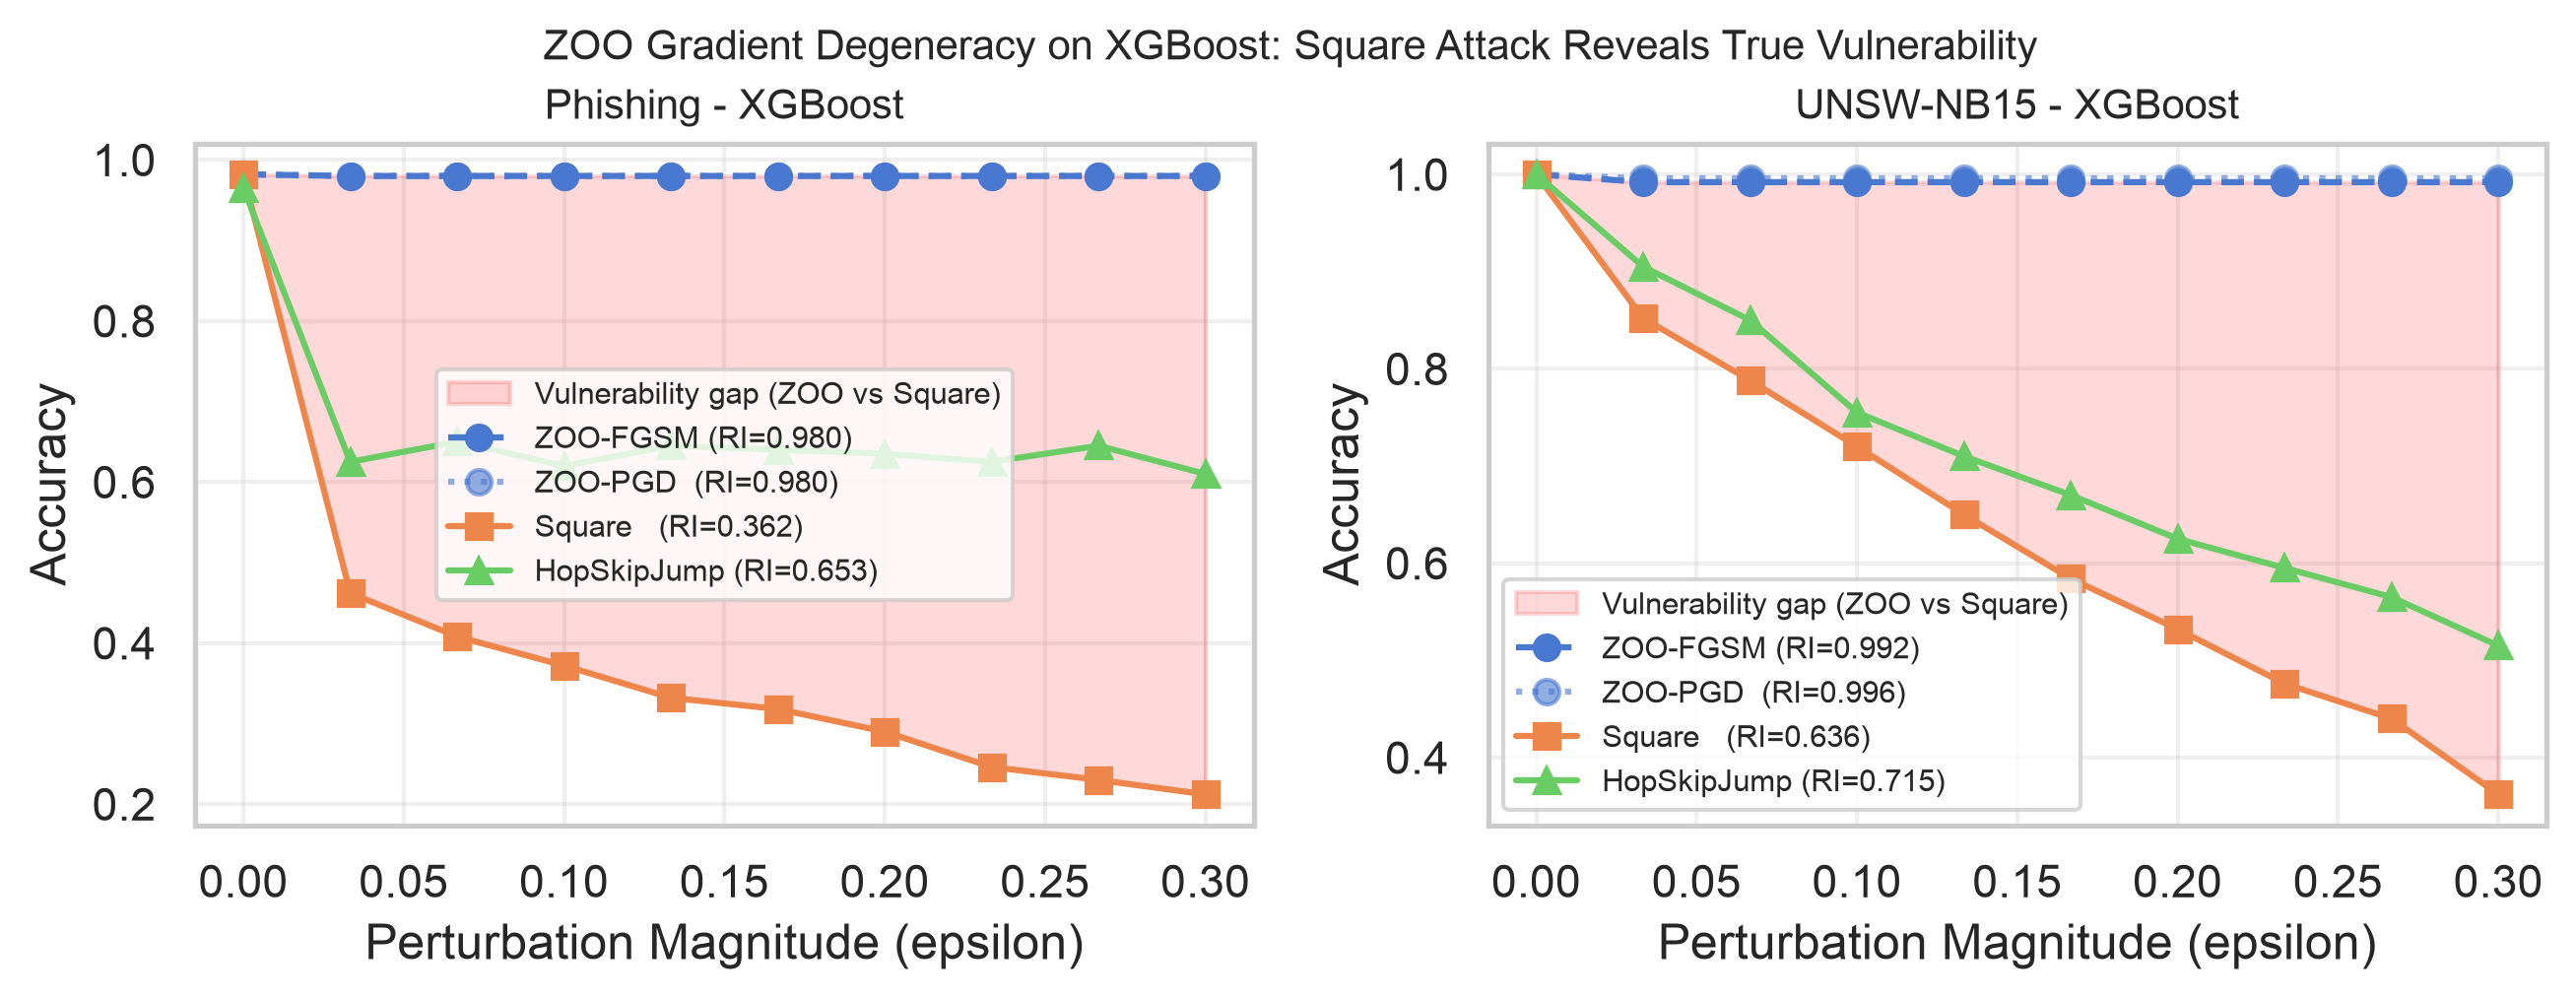
\includegraphics[width=0.85\textwidth]{../figures/xgb_attack_degeneracy.png}
  \caption{ZOO degeneracy on XGBoost: accuracy barely declines despite increasing
  $\varepsilon$, because finite-difference gradient estimates are near-zero inside
  piecewise-constant tree leaves.  Square Attack, which requires only loss values,
  reveals the true vulnerability.}
  \label{fig:degeneracy}
\end{figure}

\begin{figure}[t]
  \centering
  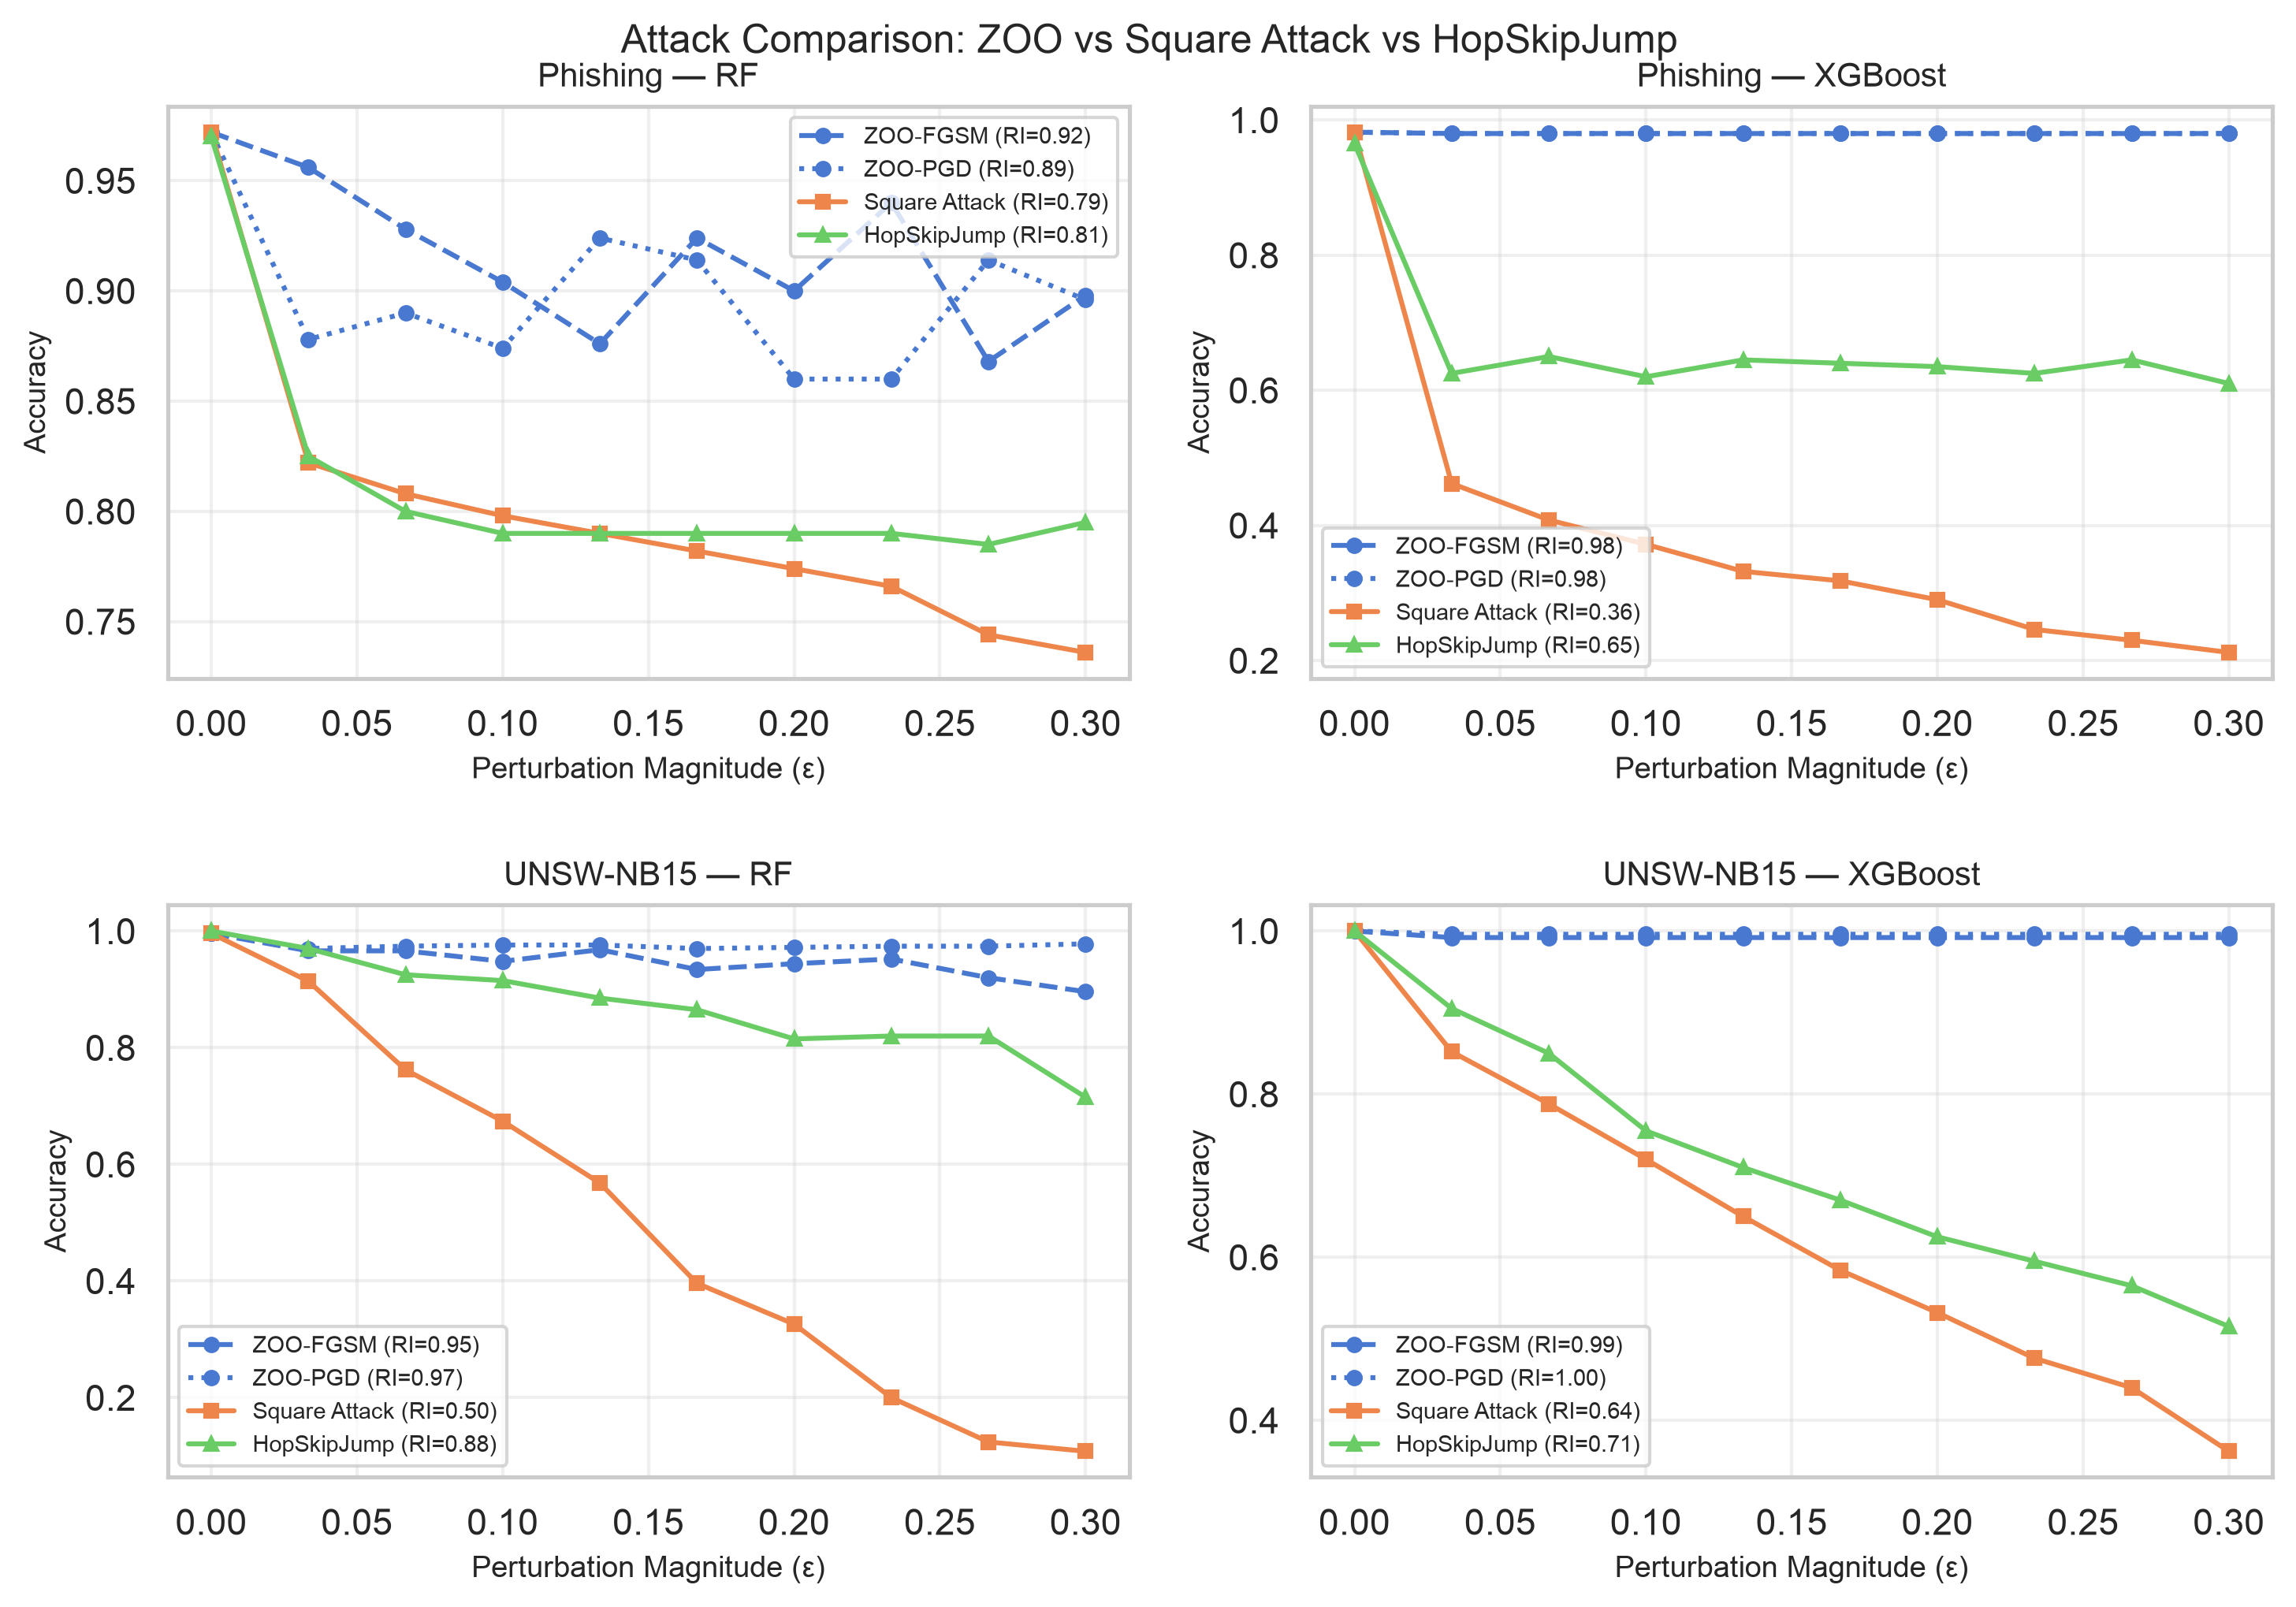
\includegraphics[width=\textwidth]{../figures/attack_comparison_curves.png}
  \caption{Accuracy vs.\ $\varepsilon$ for ZOO, Square Attack, and HopSkipJump
  on RF and XGBoost across Phishing and UNSW-NB15 datasets.}
  \label{fig:attack_comparison}
\end{figure}

\begin{figure}[t]
  \centering
  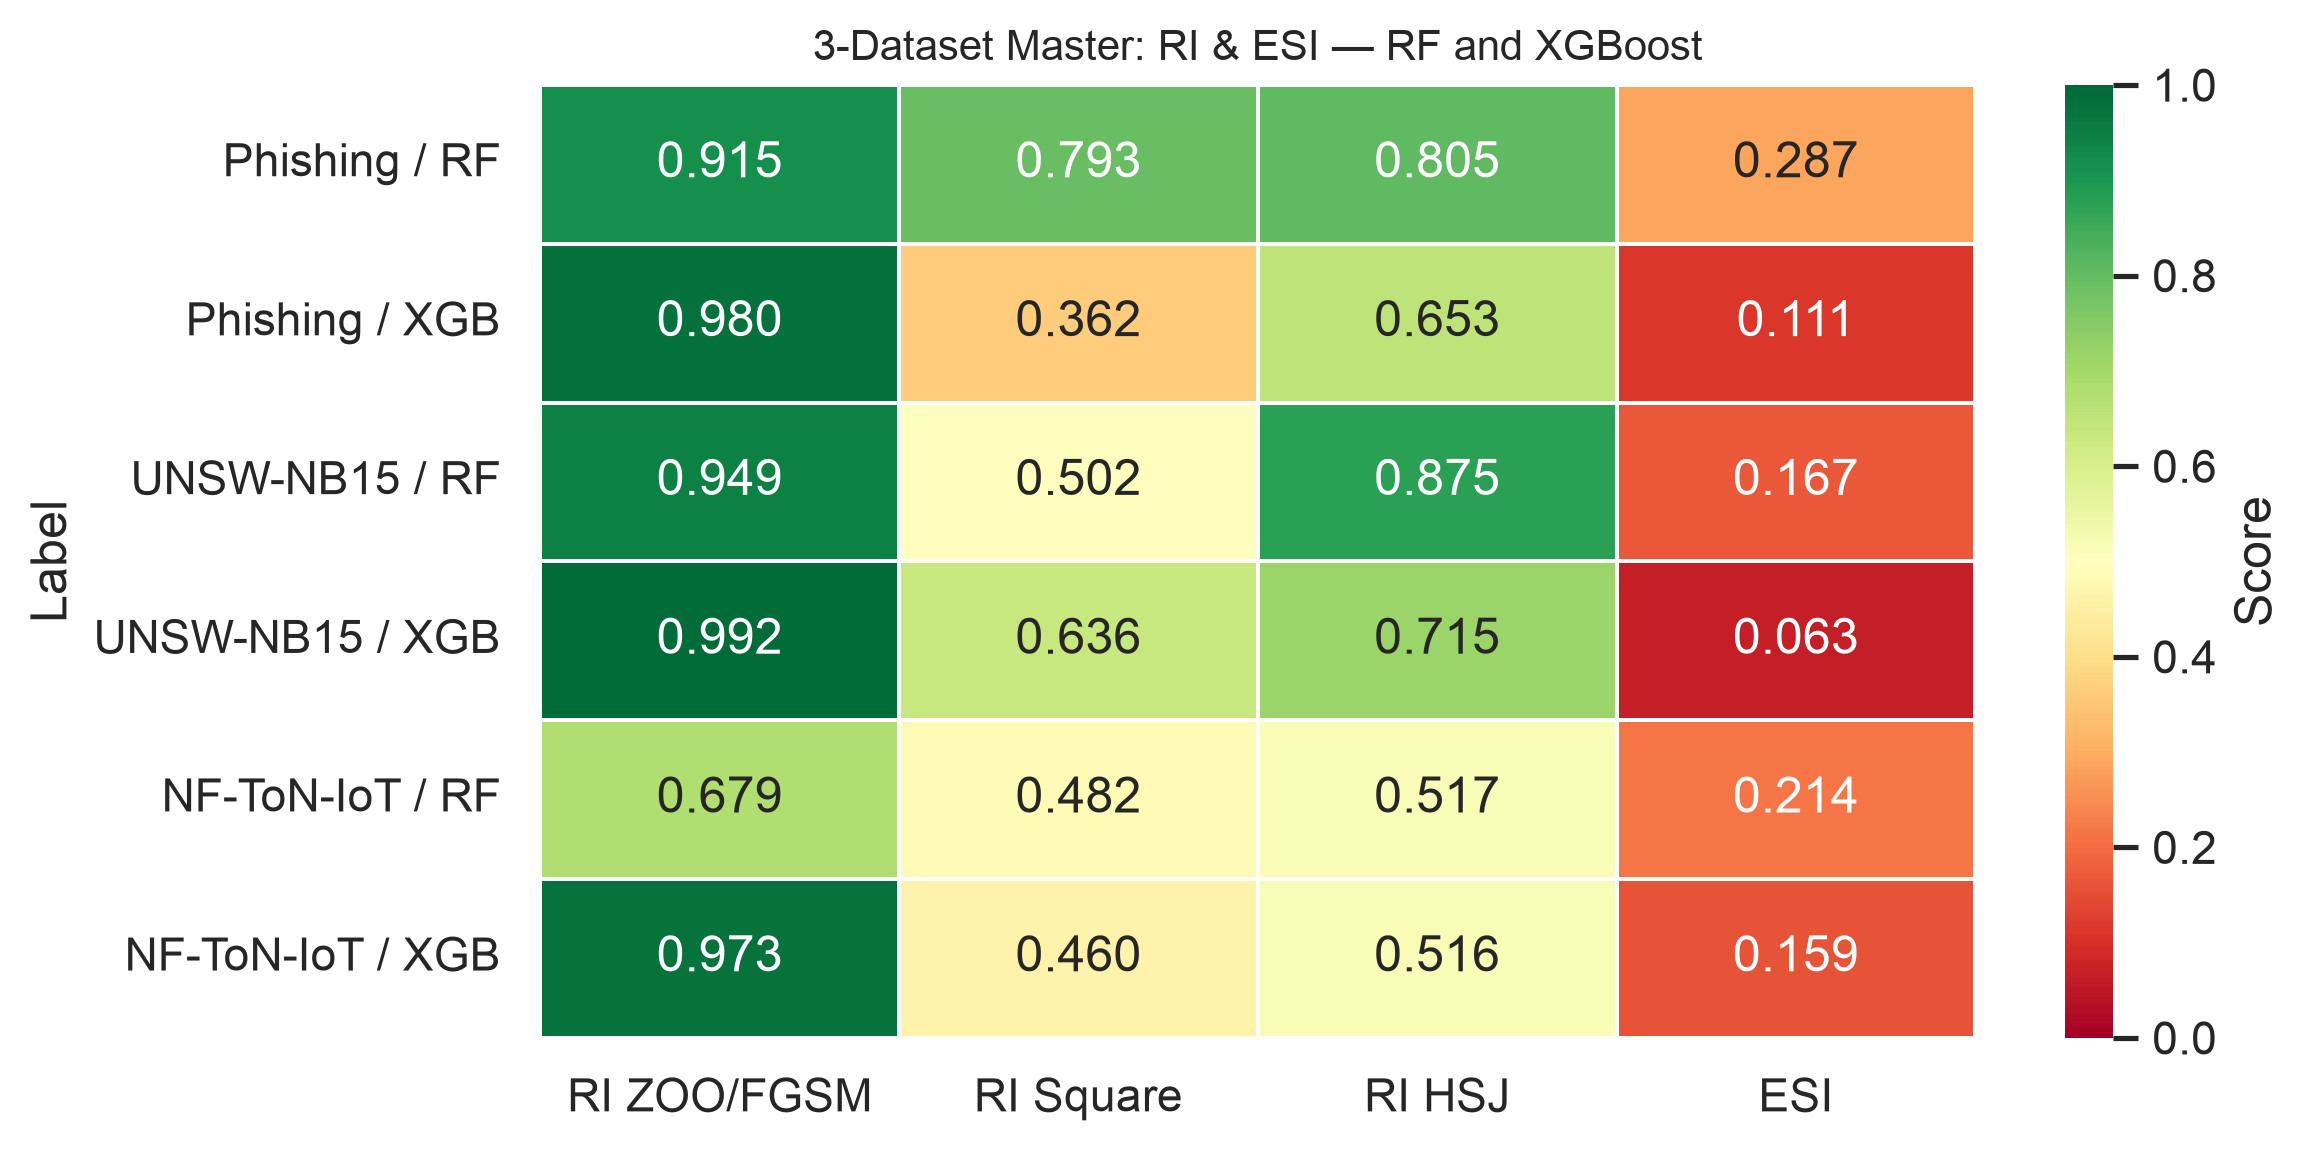
\includegraphics[width=0.85\textwidth]{../figures/master_heatmap.png}
  \caption{RI and ESI heatmap across all three datasets and tree model families.
  XGBoost consistently shows higher RI (under ZOO) but lower ESI than RF,
  illustrating the prediction-robustness vs.\ explanation-stability decoupling.}
  \label{fig:master_heatmap}
\end{figure}

% ══════════════════════════════════════════════════════════════════════════════
\section{NF-ToN-IoT: Third Dataset Evaluation}
\label{sec:toniot}
% ══════════════════════════════════════════════════════════════════════════════

Table~\ref{tab:master} includes results for NF-ToN-IoT.  Both RF and XGBoost
achieve 0.998 clean accuracy on this dataset, consistent with its highly separable
NetFlow feature structure.

A notable departure from Phishing and UNSW-NB15 is that ZOO RI for RF drops to
0.679 on NF-ToN-IoT, significantly lower than on the other datasets (0.915,
0.949).  We attribute this to the lower feature dimensionality of NF-ToN-IoT
(10 features vs.\ 48 for Phishing): with fewer features, ZOO's finite-difference
gradient estimates are more accurate, reducing the degeneracy effect.  This is a
dimensionality-dependent result and provides further evidence that ZOO degeneracy
is a function of both model architecture and feature space geometry.

XGBoost ZOO RI remains high at 0.973, confirming that the piecewise-constant
prediction surface of boosted trees dominates regardless of dimensionality.
Square Attack reduces both models to near-random (RI\,$\approx$\,0.46--0.48),
consistent with prior datasets.  ESI for RF (0.214) is between Phishing (0.287)
and UNSW-NB15 (0.167); XGBoost ESI (0.159) follows the same cross-dataset pattern.

\Cref{fig:toniot} shows the robustness curves for both models on NF-ToN-IoT.

\begin{figure}[t]
  \centering
  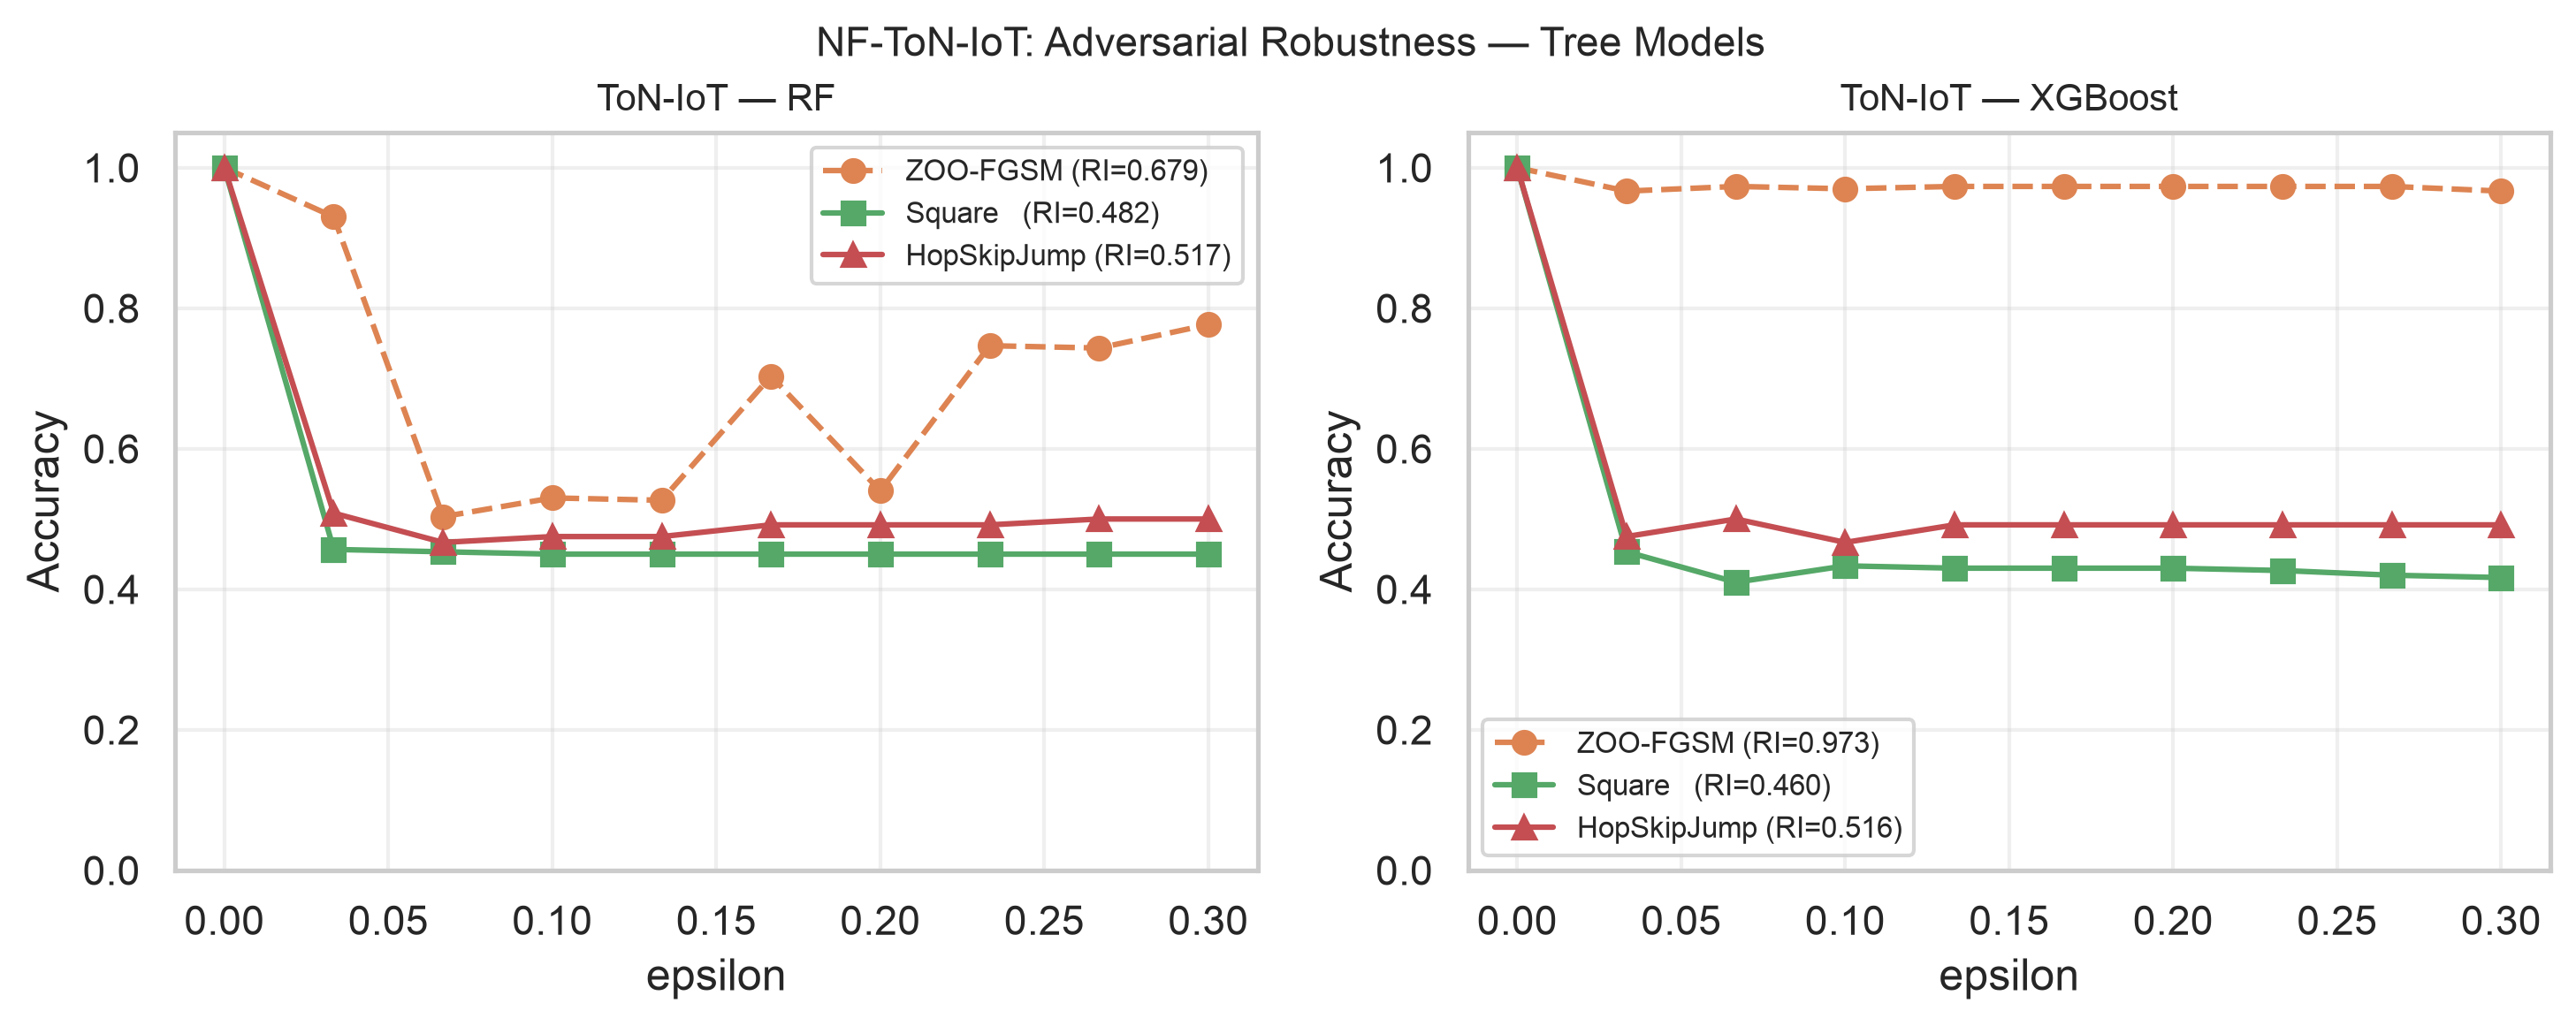
\includegraphics[width=0.85\textwidth]{../figures/toniot_robustness_curves.png}
  \caption{Adversarial robustness curves for RF and XGBoost on NF-ToN-IoT.
  ZOO is partially effective against RF (lower RI than other datasets) due to
  the lower feature dimensionality improving gradient estimate quality.}
  \label{fig:toniot}
\end{figure}

% ══════════════════════════════════════════════════════════════════════════════
\section{PGD Step-Size Ablation}
\label{sec:pgd}
% ══════════════════════════════════════════════════════════════════════════════

Our conference paper~\cite{khawarey2026empirical} observed that PGD produces
higher RI than FGSM---i.e., PGD is a \emph{weaker} attack---on both datasets.
Reviewer feedback identified this as counterintuitive, since PGD is an iterative
refinement of FGSM that should find stronger adversarial examples.

We resolve this by an ablation over PGD step sizes $\alpha \in \{0.005, 0.01,
0.02, 0.05, 0.10\}$ with fixed 10 steps, shown in \Cref{tab:pgd_ablation} and
\Cref{fig:pgd_ablation}.

\begin{table}[t]
\caption{PGD step-size ablation: Robustness Index (RI) on Phishing and UNSW-NB15
for MLP.  Higher RI indicates a weaker attack.  FGSM baseline shown for reference.}
\label{tab:pgd_ablation}
\centering
\begin{tabular}{llcc}
\toprule
Attack & $\alpha$ & RI (Phishing) & RI (UNSW-NB15) \\
\midrule
FGSM        & ---   & 0.677 & 0.713 \\
\midrule
\multirow{5}{*}{PGD (10 steps)}
            & 0.005 & 0.891 & 0.776 \\
            & 0.010 & 0.819 & 0.761 \\
            & 0.020 & 0.694 & 0.724 \\
            & 0.050 & 0.651 & 0.679 \\
            & 0.100 & 0.649 & 0.674 \\
\bottomrule
\end{tabular}
\end{table}

The ablation reveals a monotonic decrease in RI as $\alpha$ increases: PGD
becomes progressively stronger as the step size grows, converging toward and
eventually surpassing FGSM at $\alpha \geq 0.05$.  The conventional choice of
$\alpha = \varepsilon_{\max}/\text{steps} = 0.01$ is the weakest PGD
configuration tested.

The mechanism is as follows.  On z-score normalised tabular data, each PGD step
of size $\alpha=0.01$ is projected back into the $L_\infty$ ball around
$\mathbf{x}_0$.  When $\varepsilon$ is small, consecutive steps cannot accumulate
past the ball boundary, and iterative projection partially cancels gradient
progress.  FGSM's single full-budget step reaches the $L_\infty$ boundary directly
without iterative clipping interference.  This phenomenon is specific to tabular
data with z-score normalisation, where feature scales are uniform and small step
sizes are systematically ineffective.  We recommend adaptive step sizes
($\alpha = \varepsilon / \text{steps}$ per $\varepsilon$ value) for future
studies on normalised tabular data.

\begin{figure}[t]
  \centering
  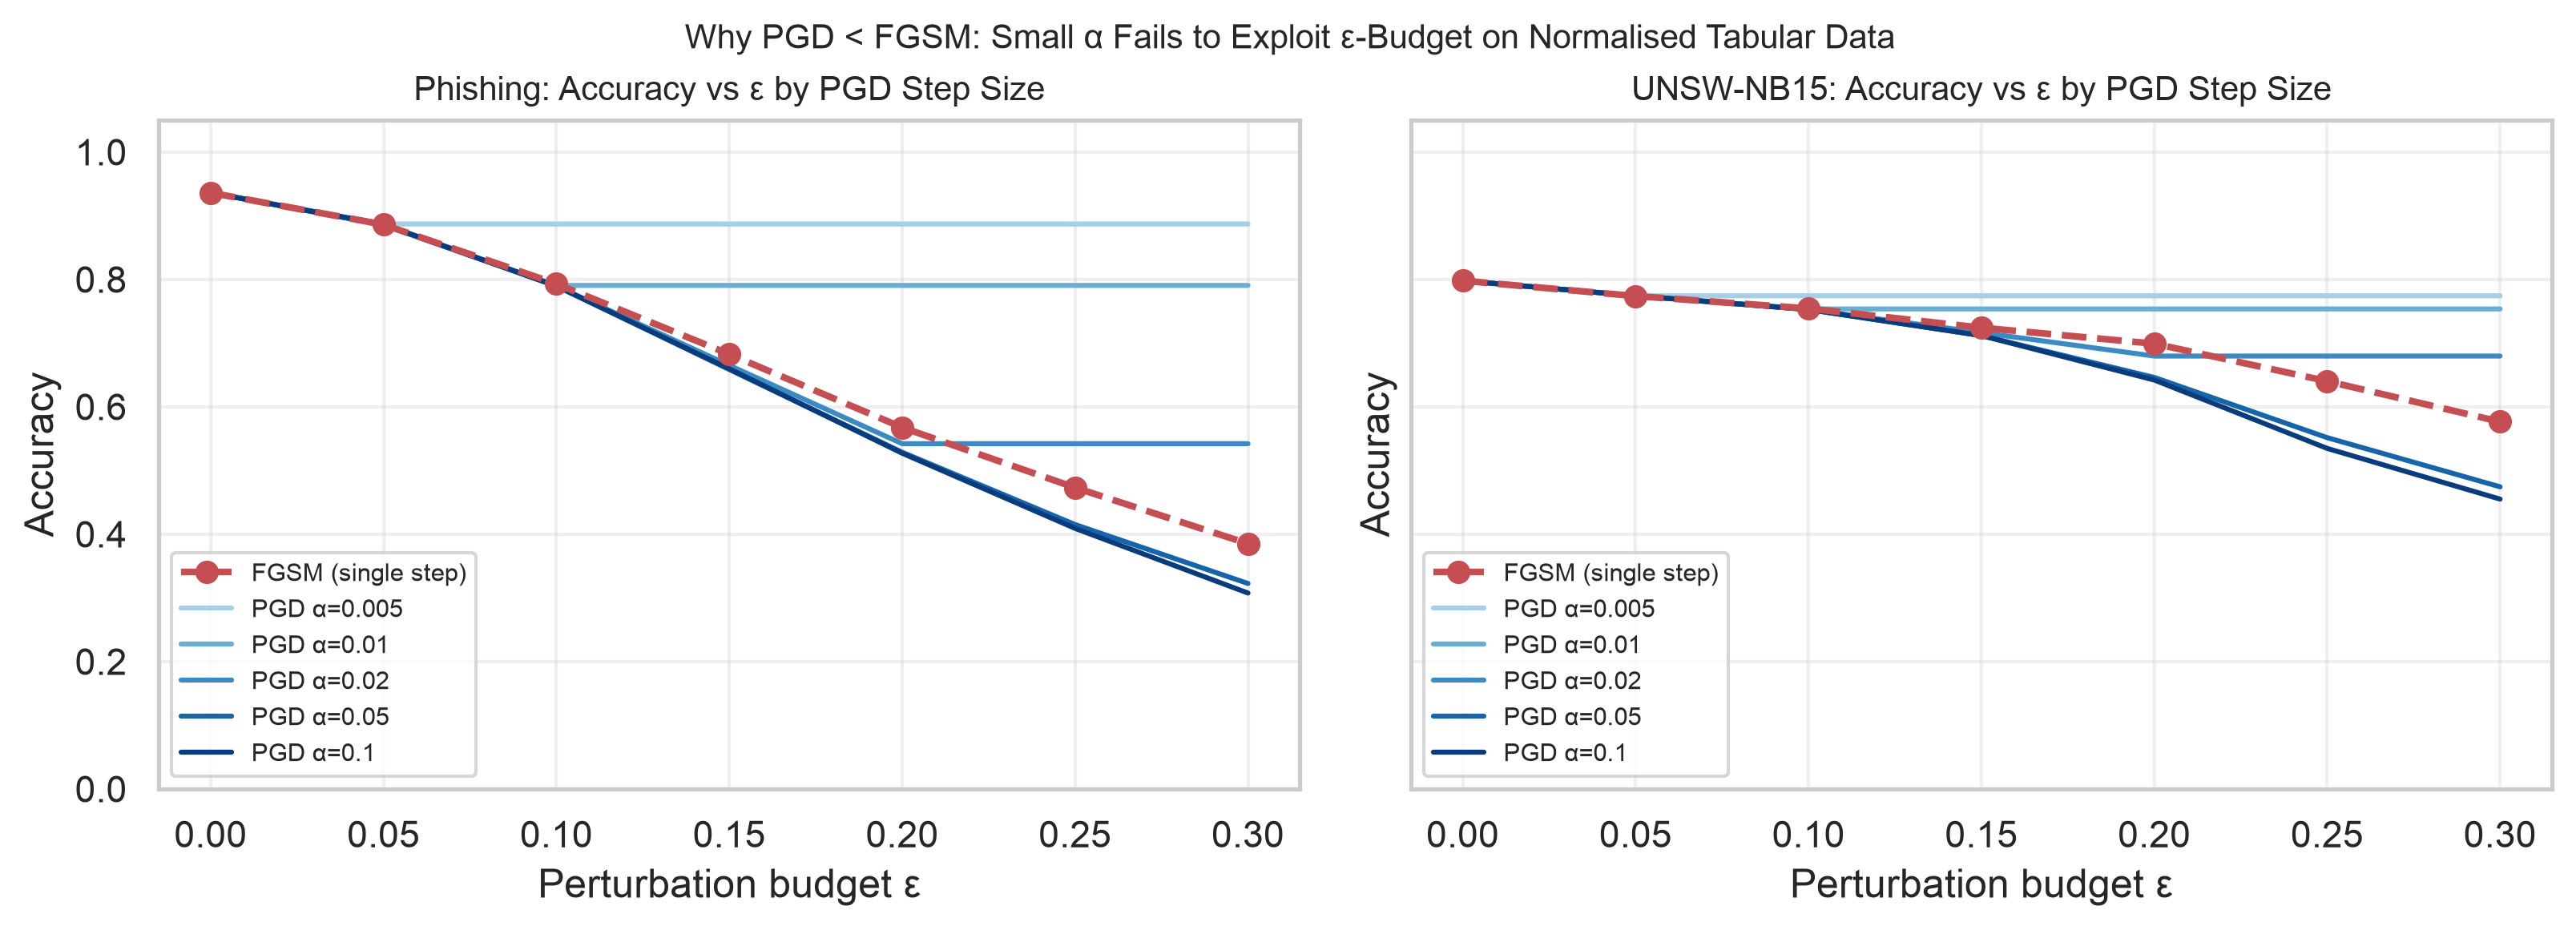
\includegraphics[width=\textwidth]{../figures/pgd_alpha_ablation_curves.png}
  \caption{Accuracy vs.\ $\varepsilon$ for FGSM and PGD at five step sizes on
  Phishing (left) and UNSW-NB15 (right).  PGD with small $\alpha$ is a weaker
  attack than FGSM; the gap closes at $\alpha \geq 0.05$.}
  \label{fig:pgd_ablation}
\end{figure}

% ══════════════════════════════════════════════════════════════════════════════
\section{Discussion}
\label{sec:discussion}
% ══════════════════════════════════════════════════════════════════════════════

\subsection{Attack Realism for Structured Security Features}

A practical concern for adversarial evaluation on tabular cybersecurity data is
whether $L_\infty$-bounded perturbations correspond to plausible adversarial
capabilities.  In phishing detection, features represent observable URL and page
structure; an attacker can realistically manipulate these (e.g.\ adding subdomains,
adjusting URL length) while preserving the phishing payload.  In network intrusion
detection, NetFlow features such as byte counts and packet rates can be shaped by
an attacker controlling the traffic source.  However, not all features are
independently actionable: some are deterministically derived from others (e.g.\
packet counts constrain byte counts), meaning unconstrained $L_\infty$ perturbations
may generate invalid feature combinations.

Our results suggest that this validity concern is more severe for gradient-based
attacks than for score-based attacks.  FGSM and PGD perturb all features
simultaneously in the gradient direction, producing combinations that may violate
network protocol constraints.  Square Attack, by contrast, perturbs random
subsets of features, and HopSkipJump searches for the nearest decision boundary,
both of which are more likely to preserve feature correlations.  The lower RI
values under Square Attack and HopSkipJump relative to ZOO may therefore partly
reflect attacks that stay closer to the feasible feature manifold, suggesting
these are more realistic threat models for operational cybersecurity evaluation.

\subsection{ESI as a Complement to RI}

Existing explanation stability metrics such as OpenXAI's RIS and
ROS~\cite{agarwal2022openxai} measure explanation faithfulness relative to model
internals.  ESI is orthogonal: it measures how explanations change specifically
under adversarial perturbation, making it a security-focused metric.  Our
cross-dataset results show that ESI is consistently ordered (XGB\,$<$\,RF across
all three datasets), suggesting it captures a stable property of the model
architecture rather than dataset-specific noise.  The decoupling between RI and
ESI---high RI does not imply high ESI---has direct operational implications: a
security team relying on SHAP explanations to triage alerts cannot assume that a
model with strong prediction robustness also provides stable explanations under
adversarial conditions.

% ══════════════════════════════════════════════════════════════════════════════
\section{Conclusion}
\label{sec:conclusion}
% ══════════════════════════════════════════════════════════════════════════════

We presented an extended empirical study of adversarial robustness and
explainability stability in tabular cybersecurity classifiers, expanding our
conference paper~\cite{khawarey2026empirical} along four dimensions: classifier
families (RF and XGBoost), attack methods (ZOO, Square Attack, HopSkipJump),
evaluation datasets (NF-ToN-IoT), and metrics (ESI).

Three findings stand out.  First, ZOO produces degenerate gradient estimates
against XGBoost, inflating apparent robustness; Square Attack reveals genuine
vulnerability with a RI gap of up to 0.64 on the same model.  This shows that
attack-method selection is not model-agnostic and that gradient-based black-box
attacks are insufficient for evaluating tree ensembles.  Second, prediction
robustness and explanation stability are decoupled: XGBoost is highly robust by
RI but poorly stable by ESI, while RF shows the opposite balance.  Third, PGD
underperforms FGSM on z-score normalised tabular data when the conventional step
size $\alpha=0.01$ is used, an artifact explained by iterative $L_\infty$
projection cancelling gradient accumulation.

Directions for future work include incorporating feature validity constraints into
the attack protocol, extending ESI to other XAI methods beyond SHAP (e.g.\ LIME),
and evaluating adversarial training as a defence for tree ensembles---for which
gradient-based training augmentation is not directly applicable.

% ── References ────────────────────────────────────────────────────────────────
\bibliographystyle{splncs04}
\bibliography{refs}

\end{document}
